% !TEX TS-program = pdflatex
% !TEX encoding = UTF-8 Unicode

% This is a simple template for a LaTeX document using the "article" class.
% See "book", "report", "letter" for other types of document.

\documentclass[11pt]{article} % use larger type; default would be 10pt


\usepackage{ulem}
\newcommand\NoIndent[1]{%
  \par\vbox{\parbox[t]{\linewidth}{#1}}%
}


\usepackage[utf8]{inputenc} % set input encoding (not needed with XeLaTeX)

%%% Examples of Article customizations
% These packages are optional, depending whether you want the features they provide.
% See the LaTeX Companion or other references for full information.

%%% PAGE DIMENSIONS
\usepackage{geometry} % to change the page dimensions
\geometry{a4paper} % or letterpaper (US) or a5paper or....
% \geometry{margin=2in} % for example, change the margins to 2 inches all round
% \geometry{landscape} % set up the page for landscape
%   read geometry.pdf for detailed page layout information

\usepackage{graphicx} % support the \includegraphics command and options

% \usepackage[parfill]{parskip} % Activate to begin paragraphs with an empty line rather than an indent

%%% PACKAGES
\usepackage{booktabs} % for much better looking tables
\usepackage{array} % for better arrays (eg matrices) in maths
\usepackage{paralist} % very flexible & customisable lists (eg. enumerate/itemize, etc.)
\usepackage{verbatim} % adds environment for commenting out blocks of text & for better verbatim
\usepackage{subfig} % make it possible to include more than one captioned figure/table in a single float
% These packages are all incorporated in the memoir class to one degree or another...

%%% HEADERS & FOOTERS
\usepackage{fancyhdr} % This should be set AFTER setting up the page geometry
\pagestyle{fancy} % options: empty , plain , fancy
\renewcommand{\headrulewidth}{0pt} % customise the layout...
\lhead{}\chead{}\rhead{}
\lfoot{}\cfoot{\thepage}\rfoot{}

%%% SECTION TITLE APPEARANCE
\usepackage{sectsty}
\allsectionsfont{\sffamily\mdseries\upshape} % (See the fntguide.pdf for font help)
% (This matches ConTeXt defaults)

%%% ToC (table of contents) APPEARANCE
\usepackage[nottoc,notlof,notlot]{tocbibind} % Put the bibliography in the ToC
\usepackage[titles,subfigure]{tocloft} % Alter the style of the Table of Contents
\renewcommand{\cftsecfont}{\rmfamily\mdseries\upshape}
\renewcommand{\cftsecpagefont}{\rmfamily\mdseries\upshape} % No bold!

%%% END Article customizations


\usepackage{verbatim}
\usepackage{amsmath}

\usepackage{pdfpages}

\title{Work Log for October}
\author{Logan Brown}
%\date{} % Activate to display a given date or no date (if empty),
         % otherwise the current date is printed 


\begin{document}
\maketitle
\tableofcontents

\newpage


\section{Goals for the Month}
As of Sept 30th
%Old Goals
\begin{enumerate}
\item Find out what causes some of the probabilties to go outrageously high
\item Use the Simulated Yeast Genome, compare to the Ecoli genome
\item If possible, NSE Patch
\item Debugging Thoughts
\end{enumerate}
%\begin{enumerate}
%\item Find out what causes some of the probabilties to go outrageously high
%\item Compare Differences in the Code
%\item Compare Genomes
%\item Look at the change in the proposed Phi distribution over time
%\item Look at stddev(phi)
%\item Make a git repository for my scripts
%\item NSE Patches
%\end{enumerate}


\section{Progress/Notes}

\subsection{Code notes}

\subsubsection{my.logdmultinomCodOne.r}

\begin{verbatim}
tmp.phi <- rep(phi, naa)
xm <- matrix(cbind(1, tmp.phi * reu13.df.aa$Pos), ncol = 2)
baamat <- matrix(-baa, nrow = 2, byrow = TRUE)
xm%*%baamat
\end{verbatim}

Phi is the expression level of each codon. Naa is the number of times that each amino acid appears in each codon. So tmp.phi is essentially stretched out phi. reu13.df.aa\$Pos is the position information (sorted increasing by value). 

baamat is the codon specific information, baamat[1,1] is the mutation bias, baamat[2,1] is the odds ratio. So xm\%*\%baamat is $1*\mbox{mutation bias}+\mbox{odds}*\mbox{position}*\mbox{phi})$

\begin{verbatim}
Browse[1]> head(phi)
      aaeB       aaeR        aas        aat       accA       accB 
 0.8974192  3.2587638  1.7777326  0.9867905  2.4253851 49.4914945 
Browse[1]> head(naa)
aaeB aaeR  aas  aat accA accB 
  30   14   27    7   11    8 
Browse[1]> head(tmp.phi)
     aaeB      aaeB      aaeB      aaeB      aaeB      aaeB 
0.8974192 0.8974192 0.8974192 0.8974192 0.8974192 0.8974192 
Browse[1]> head(xm)
     [,1]       [,2]
[1,]    1   7.179353
[2,]    1  27.819994
[3,]    1 121.151588
[4,]    1 128.330941
Browse[1]> baamat
             [,1]
[1,] -0.890071751
[2,]  0.001831086
Browse[1]> head(xm%*%baamat)
           [,1]
[1,] -0.8769257
[2,] -0.8391310
[3,] -0.6682328
[4,] -0.6550868
\end{verbatim}



\subsection{Find out what causes some of the probabilties to go outrageously high}

It may not be a gradual process?

When I ran the NSE model on Ecoli after the oct20 config file change, element 571 of the lpProp vector was the one that proposed NaN. Below, I've included the final 20 values of lpProp 571, and its neighbors, 570 and 572. Its behaviors are not that weird by comparison.

\begin{verbatim}
      	lpProp 570  lpProp 571 lpProp 572
[4177,]  -439.0460   -73.72289  -62.74278
[4178,]  -436.8223  -204.74990  -63.29419
[4179,]  -435.2346   -64.24408  -62.59052
[4180,]  -436.0235   -73.35364  -64.13391
[4181,]  -438.3667   -67.98921       -Inf
[4182,] -2649.8670   -72.62635  -63.57204
[4183,]  -435.5443  -115.24960 -134.97510
[4184,]  -435.2912        -Inf  -65.44034
[4185,]  -436.1059  -340.63310  -65.11169
[4186,]  -589.3728   -68.32954  -67.40303
[4187,]  -436.4503   -81.33534  -82.93474
[4188,]  -436.3286   -72.06965       -Inf
[4189,]  -438.5207   -63.91668 -120.27640
[4190,]  -435.6769 -1054.61800       -Inf
[4191,]  -435.5219 -1945.30800  -66.77650
[4192,]  -437.3907   -77.26036  -62.84463
[4193,]       -Inf   -65.85979  -62.55160
[4194,]  -442.1116   -68.60126  -63.96031
[4195,]  -438.5858        -Inf -572.40770
[4196,]  -437.3305        -Inf  -67.74666
\end{verbatim}

At the time, the current and previous drawscale were 10.04997, which are higher than most, but outrageously high. Others in that group had similar and higher scales, and none of those crashed the code. In fact, their lp.c.raw values run the gamut \textit{(including 0?)}

\begin{verbatim}
Browse[1]> cbind(scales[which(scales>9.5)], lp.c.raw[which(scales>9.5)])
           [,1]       [,2]
 [1,] 10.049972        NaN
 [2,]  9.647973 -1.2280060
 [3,] 10.049972 -1.8911363
 [4,] 10.049972  0.0000000
 [5,]  9.860494 -0.6880676
 [6,]  9.647973 -5.4668636
 [7,] 10.468721       -Inf
 [8,] 10.904917       -Inf
 [9,] 10.468721 -0.3495275
[10,] 10.468721  0.0000000
\end{verbatim}

\subsubsection{0s in lp.c.raw}

There doesn't seem to be strong correlation between the lp.c.raw and the 0 values proposed in lp.c.raw. They do have 4 values in common (2174, 2175, 2181, and 2185), but the other scales vary from 1.6 to 10.4.

\begin{verbatim}
Browse[1]> which(scales>9)
 [1]  223  339  352  353  467  534  571  644  652  657  705  890  916 1239 1709
[16] 1723 1734 1833 1884 2003 2049 2153 2174 2175 2181 2185 2187
Browse[1]> which(lp.c.raw==0)
 [1]  119  352  587  600  651  705  733  756  885 1124 1378 1410 1528 1562 1694
[16] 1880 1906 1963 1982 2152 2165 2174 2175 2178 2181 2185 2190
Browse[1]> scales[which(lp.c.raw==0)]
 [1]  7.269945  9.087431  7.269945  3.573323  2.858659 10.049972  8.039977
 [8]  7.888395  8.039977  8.374976  5.815956  6.979147  6.058287  7.572859
[15]  6.979147  7.572859  1.623127  6.979147  2.286927  7.572859  7.269945
[22] 10.468721  9.087431  7.269945  9.466074  9.087431  6.310716
\end{verbatim}


\subsubsection{Two -Infs in a Row?}

\sout{It's possible that the absurd values are being proposed because the previous two values are both -Inf ($ln(-\infty)=0$)}

Confirmed that this is not a problem. The code can propose at least 9 -Infs in a row without crashing.



\subsubsection{Codon Length / Lack of Information?}

Here's a few of the ecoli genes and amino acids that led to NaN
\begin{itemize}
\item evgA - 205 codons, G Glycine (4 synomyms)
\item yhdT - 80 codons, R Arginine (6 synonyms)
\item gnsA - 58 codons, Q Glutamine (2 synonyms)
\end{itemize}






\newpage
\subsection{Compare Differences in the Code}
\begin{verbatim}
my.coef.r
my.drawPhiConditionalAllPred.r
my.drawPhiConditionalAll.r
my.estimatePhiOne.r
my.fitMultinomOne.r
my.logdmultinomCodOne.r
my.objectivePhiOne.Lfp.r
my.objectivePhiOne.nlogL.r
my.objectivePhiOne.nlogphiL.r
my.objectivePhiOne.phiLfp.r
my.pPropTypeNoObs.lognormal_bias.r
plotbin.r
plotmodel.r
simu.orf.r
\end{verbatim}


Codes where NSE and ROC are the same, or incredibly similar:
\begin{verbatim}
my.coef.r
my.estimatePhiOne.r
\end{verbatim}

Codes where NSE and ROC differ:
\begin{verbatim}
my.drawPhiConditionalAllPred.r
my.drawPhiConditionalAll.r
\end{verbatim}





\newpage
\subsection{Compare Genomes}

\subsubsection{The Gist}

I haven't touched this section in two weeks or so, so it's fairly outdated.

The gist is that Yeast tends to have scales hovering around 3.5-4 for ROC and NSE.

Ecoli tends to have scales hovering around .7, at least for ROC. For NSE, it may center closer to 4 as well? Curious. Average ROC scale never went above 1.

\subsubsection{Use Sections of the Simulated Yeast Genome}
I ran one 5th of the yeast genome(section1.fasta, section1.csv) and it FINISHED. but... not well.

See the results in data/10.01.yeastnse.*

\begin{itemize}
\item It took just over 30 hours to finish\\
started at: 2014-10-01 15:57:54\\
finished at: 2014-10-02 22:08:56 

\item The proposed phi values are still outrageously too high. The final proposed phi had mean value 2766786.09545948

\item Still proposing some 0 (-Inf) values for lpProp. At most, around 45-49 Inf per run.

\item Xobs (the original phi values) are generally much lower than the results of run

\item The values are not very accurate. They don't resemble the known phi values.

\end{itemize}


\subsubsection{Crashed Yeast Run}

The vast vast majority of the phi values being proposed are fine. -Inf values are throwing it off. 
10/22 Note: Due to the config file change (See Patch 1 and "look at stddev(phi)"), I'm discrediting these values.


\subsubsection{E. Coli genome}

A LARGE NSE RUN OF THE E. COLI GENOME RAN TO COMPLETION.
10/22 Note: Due to the config file change (See Patch 1 and "look at stddev(phi)"), I'm discrediting these values.








\subsection{Look at the change in the proposed Phi distribution over time}

Trying to find a nice way to look at these.

%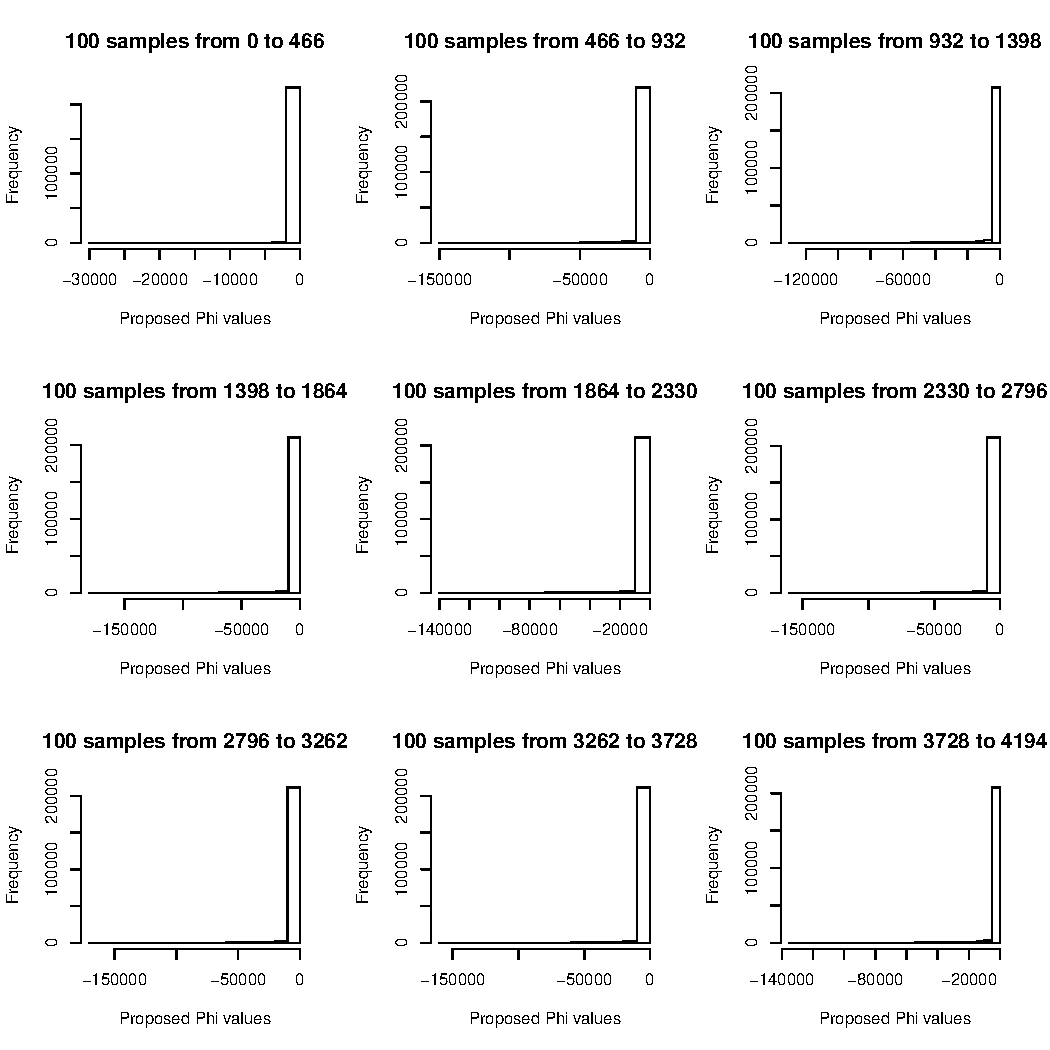
\includepdf[pages={1}]{data/NSE-yeast-phiHistory.pdf}

\newpage
\subsection{Look at stddev(phi)}

I have a run going that is tracking the scales of the MCMC for the phi values.

Since the scale of the MCMC should be about the Standard Devation of Phi, we'll see what happens.

\subsubsection{Scale reset}
PROBLEM:
The ROC model has different Phi scales for each gene. The NSE model keeps all the scales the same between different genes. That could be contributing to the problem? \sout{I think this is caused by the opatch we wrote that replaces Wei-Chen's scaling by .5  with subtracting out log(DBL\_MAX).}

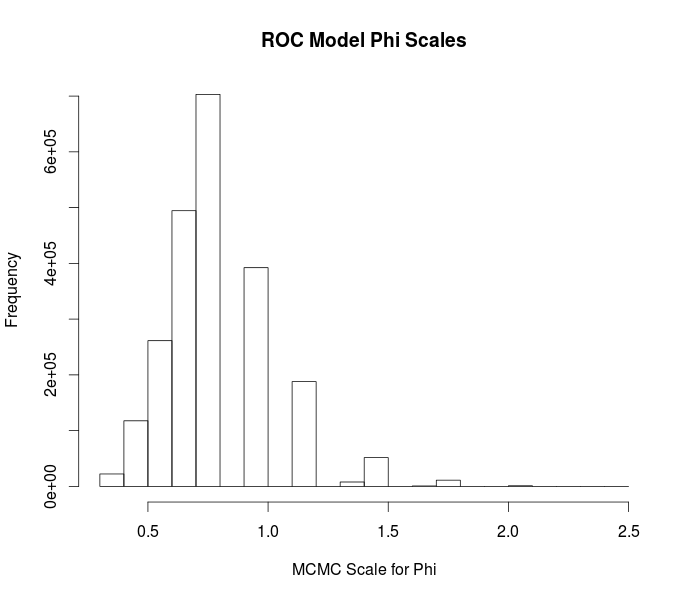
\includegraphics[width=0.5\textwidth]{data/oct10-roc-scalehist.png}
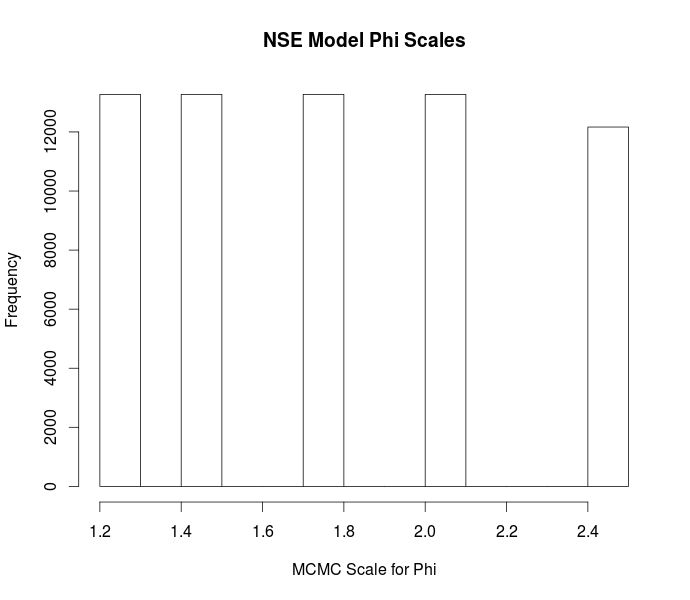
\includegraphics[width=0.5\textwidth]{data/oct10-nse-scalehist.png}

\textbf{Every 6th time that the scale is updated, the code resets all the scales to 1. This definitely happens in Yeast (NSE and ROC), and it definitely happens for NSE (Yeast and Ecoli). Does it happen in ROC-Ecoli? Yes, confirmed.}

Also, Cedric says the number 6 is a result of the inputs. It has to do with the fact that my runs have been doing 50 samples between convergence checks and 10000 . I'm going to play with config.r to see this effect. (Confirmed).

Theory: length(.cubfitsEnv\$DrawScale\$phi) is $$\frac{\mbox{Number of Samples between Convergence Checks}}{100} + 1.$$

Every time that the code checks for convergence, it reinitializes some values, and causes the problem.

By changing my values in config.r so that the code never checks for convergence (and therefore, never resets the scale), we get the following picture (left, before the change, right after the change)

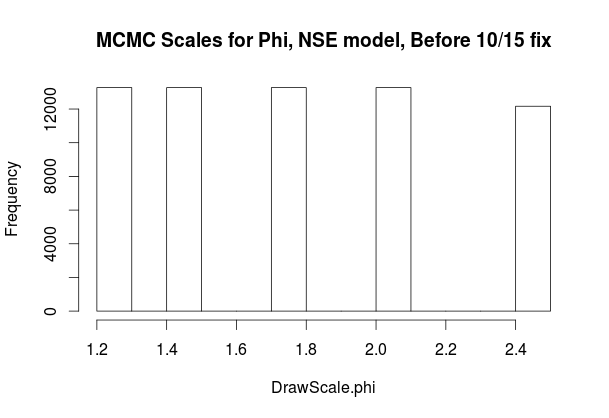
\includegraphics[width=0.5\textwidth]{data/oct15-phiscales-before_change.png}
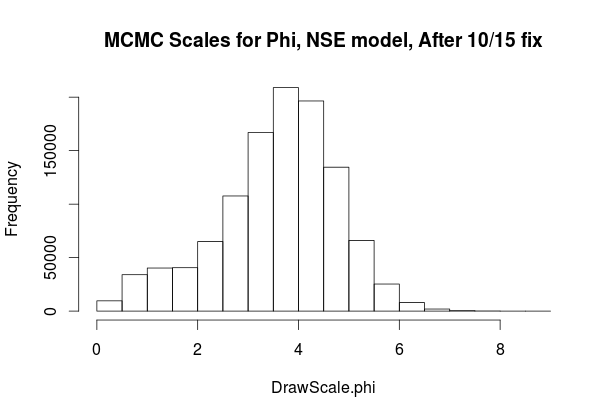
\includegraphics[width=0.5\textwidth]{data/oct15-phiscales-after_change.png}

\begin{itemize}
\item It's worthy of note that this is the second time a run of the NSE model on the Yeast genome has run to completion. Since this has happened in the past, I don't want to entirely attribute the successful run to the removal of the scaling reset, but this is some evidence. This may have been the problem preventing a successful NSE run.

\item I expect the ROC model to have a similar but less dramatic change. The former phiscale values were all ones that were within $(1.2)^i(0.8)^j$ where $i, j, i+j \in \{0, 1,...,6\}$. The ROC model should have more varied scaling terms (likely a Normal distribution)

\item It appears that the "proper" distribution of the phi scales is roughly a normal distribution that is slightly biased towards lower values. The whole set has mean=3.570621 and $\sigma$=1.196958.


\item but this seems odd to me. If the scale should be something like 4, but it was being artificially held back to $[0,2.48832]$, why was it therefore proposing NaN values? Shouldn't a LARGER scale make us more likely to propose impossible phi values? A small (and indeed, a very strangely behaving) scale should only prevent us from making progress, it shouldn't push us over some sort of cliff in the parameter space.
\end{itemize}


\subsubsection{Graph scale vs logprob(phi)}

The graphs from October 24th fall under the same accident described in the following section. They are the log probabilities of accepting a proposed phi value, NOT the proposed phi values.
This will be mended.

The graphs are still included in the data folder under the name 
\begin{verbatim}
data/S_phi-vs-lpPhi-<Model><Genome>-1000.png
\end{verbatim}

%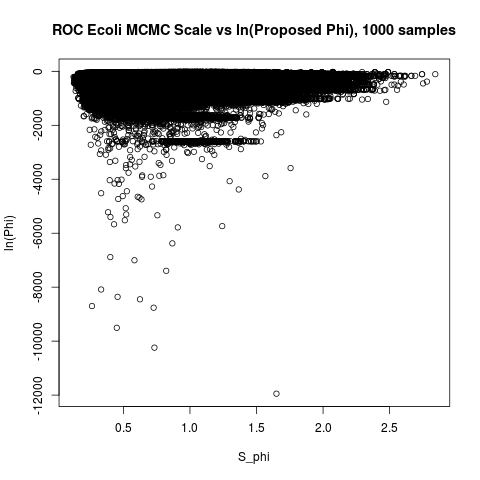
\includegraphics[width=0.5\textwidth]{data/S_Phi-vs-lpPhi-RocEcoli-1000.png}
%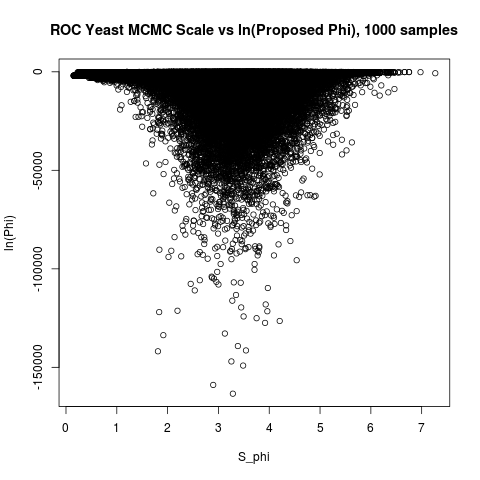
\includegraphics[width=0.5\textwidth]{data/S_Phi-vs-lpPhi-RocYeast-1000.png}
%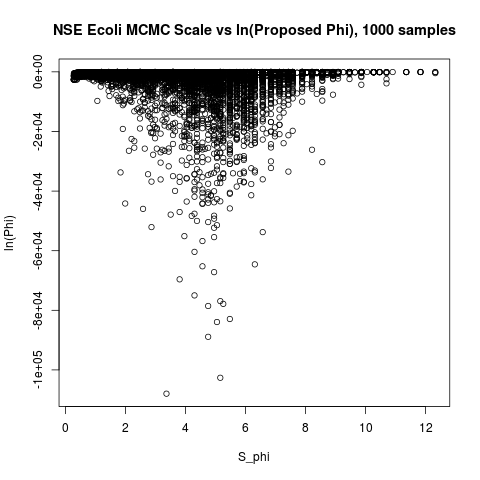
\includegraphics[width=0.5\textwidth]{data/S_Phi-vs-lpPhi-NseEcoli-1000.png}
%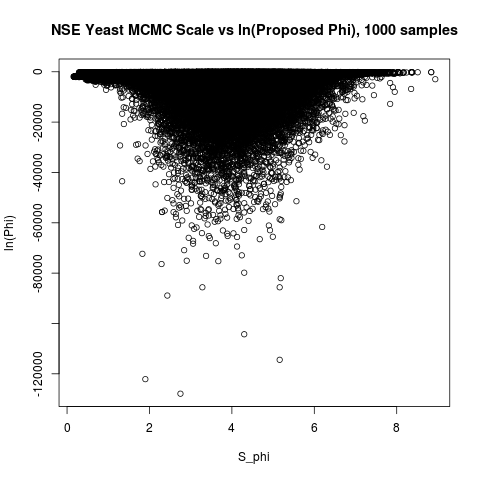
\includegraphics[width=0.5\textwidth]{data/S_Phi-vs-lpPhi-NseYeast-1000.png}




\newpage
\subsection{Look at (Current State - Proposed Phi)}

First runs, I subtracted the log probability of the proposed state from the log probability of the current state. This was a mistake, I should have been subtracting the log(proposed phi) from log(current phi). This error has been corrected. 

These graphs are still in the data folder, under the name 
\begin{verbatim}
data/oct27-<Model><Genome>-lpCurr-lpProp.png
\end{verbatim}
Where model is R for ROC or N for NSE, and genome is E for Ecoli or Y for Yeast.

%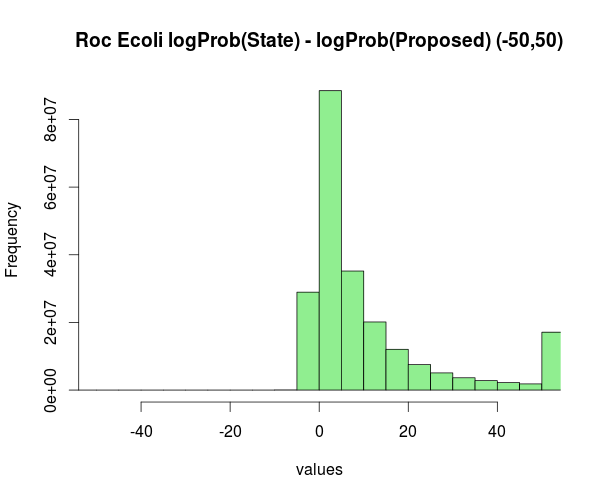
\includegraphics[width=0.5\textwidth]{data/oct27-RE-lpCurr-lpProp.png}
%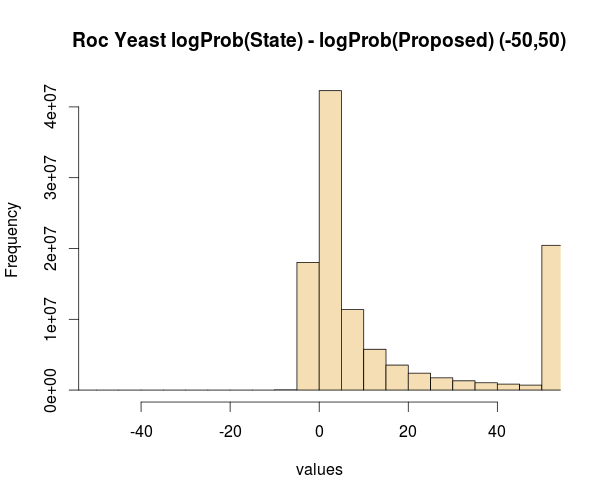
\includegraphics[width=0.5\textwidth]{data/oct27-RY-lpCurr-lpProp.png}

%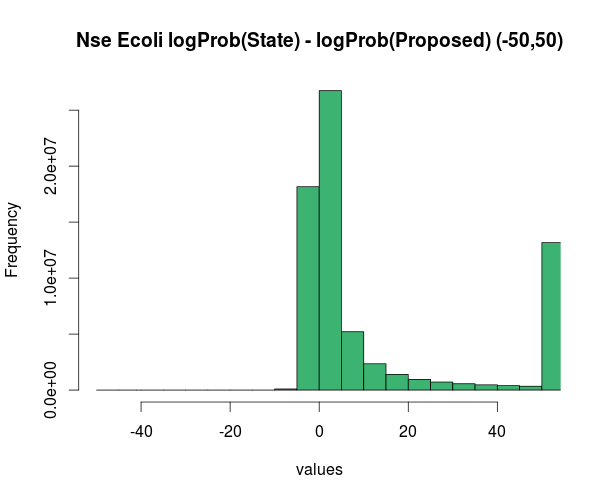
\includegraphics[width=0.5\textwidth]{data/oct27-NE-lpCurr-lpProp.png}
%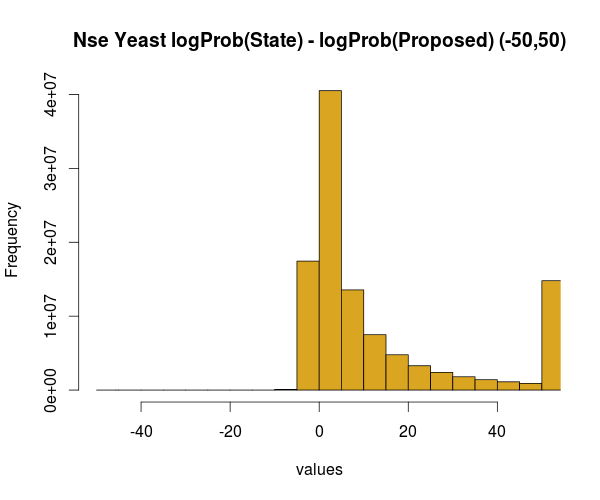
\includegraphics[width=0.5\textwidth]{data/oct27-NY-lpCurr-lpProp.png}


\newpage
\subsection{Analyse Successful NSE Yeast Run}

NSE Ecoli also ran after the patch, but the estimated phi versus the 'true' phi values had a negative correlation. We're focusing on the NSE Yeast for now, to see how things are running.

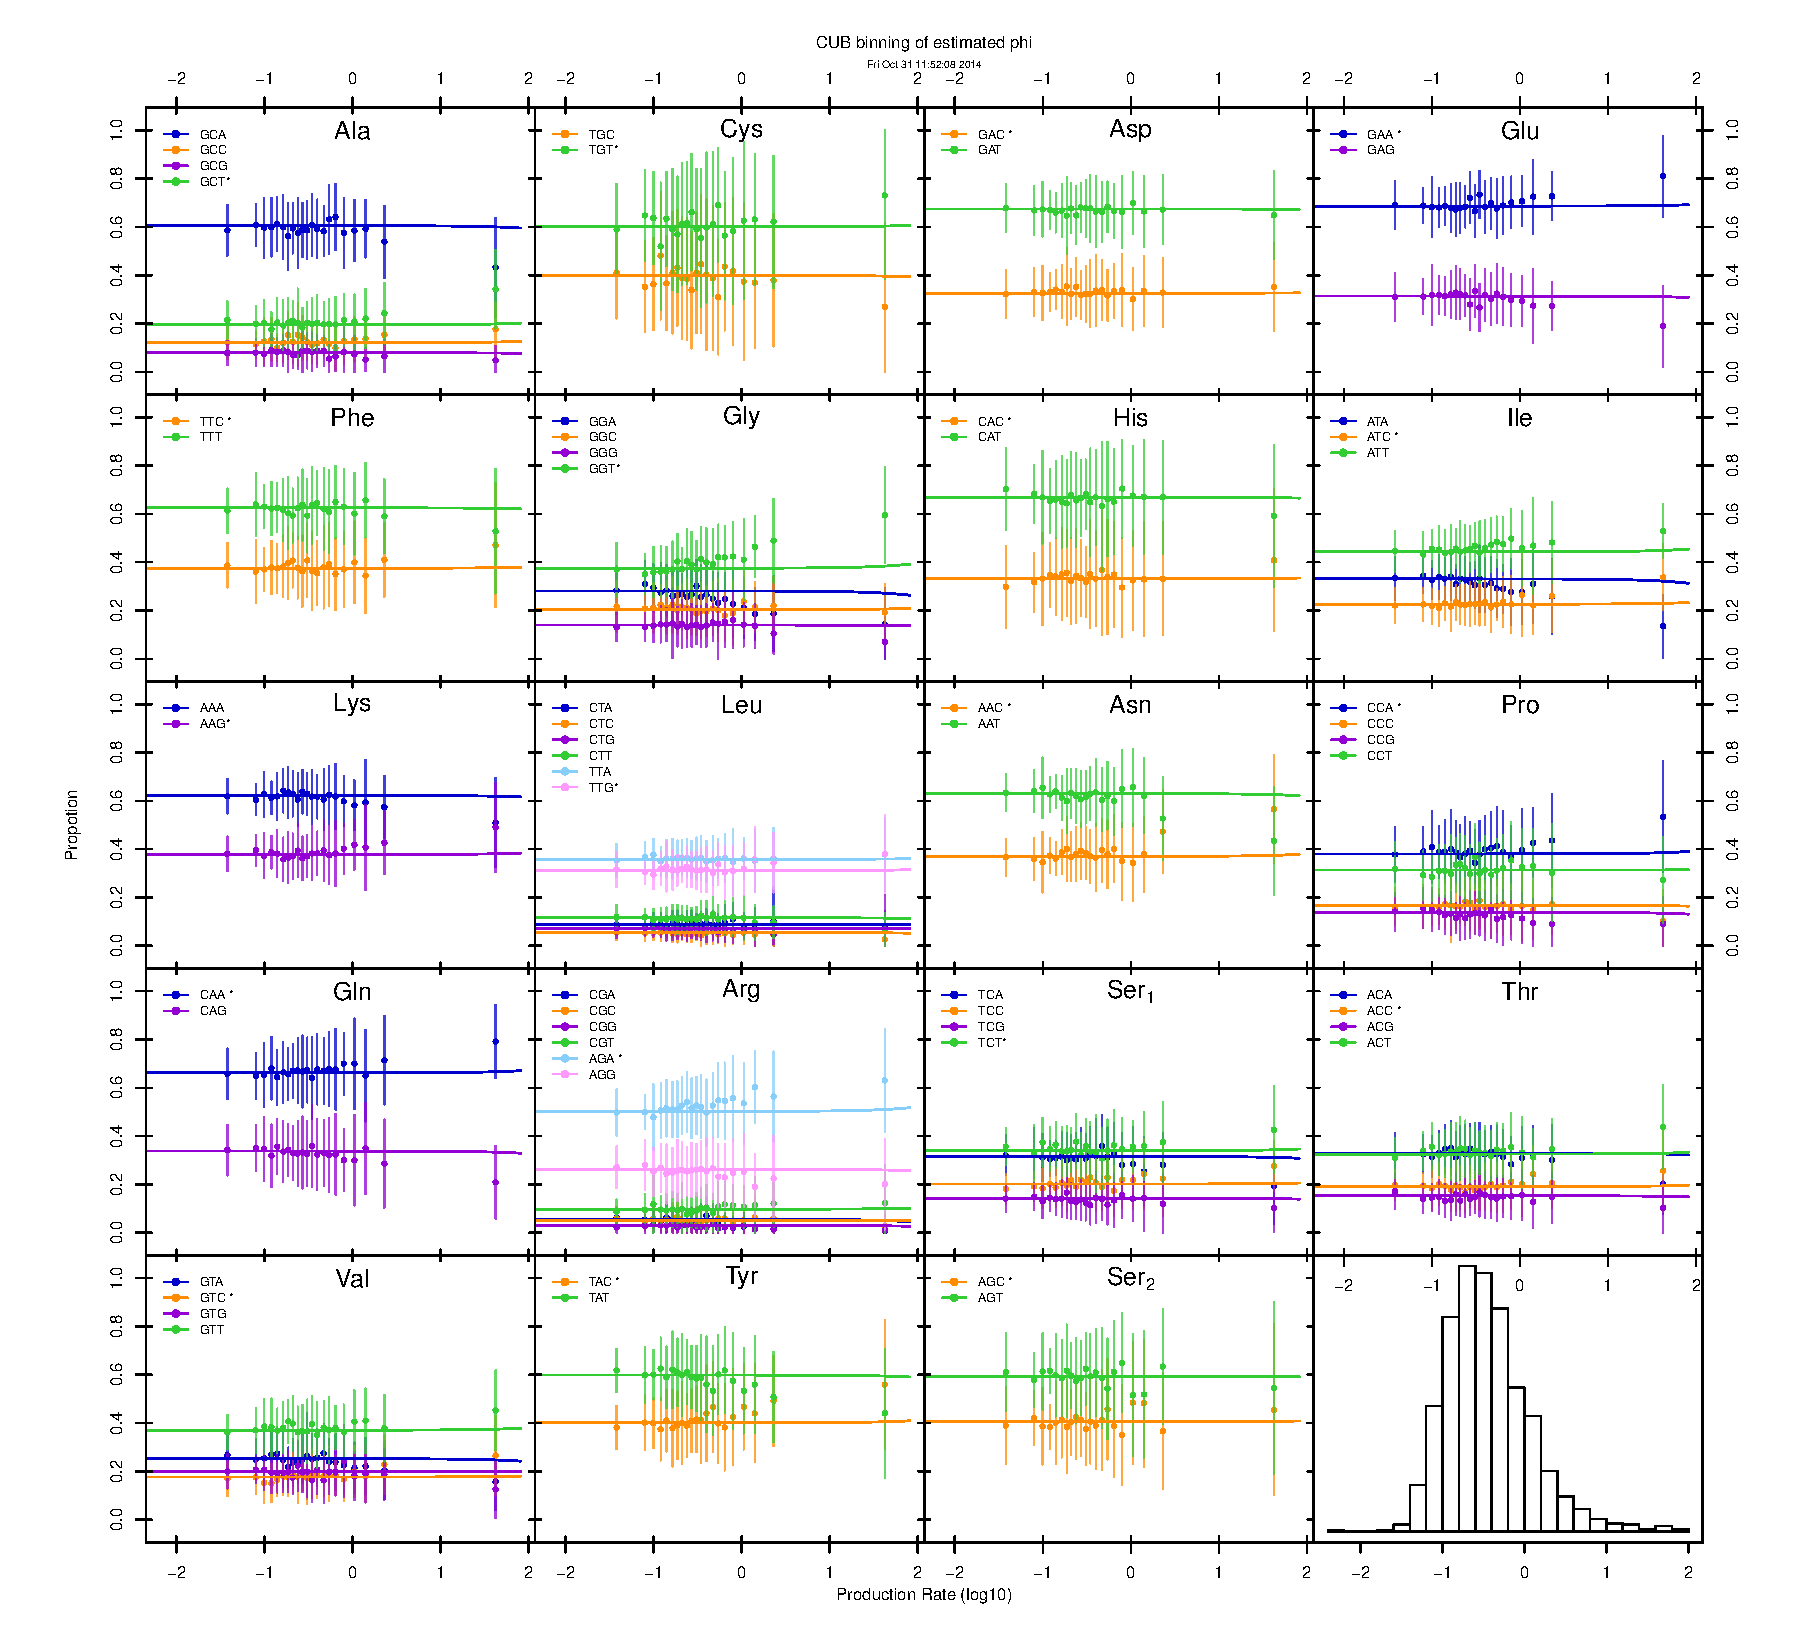
\includepdf[pages={1}]{data/oct31_CUB_est_bin_NseYeast.pdf}
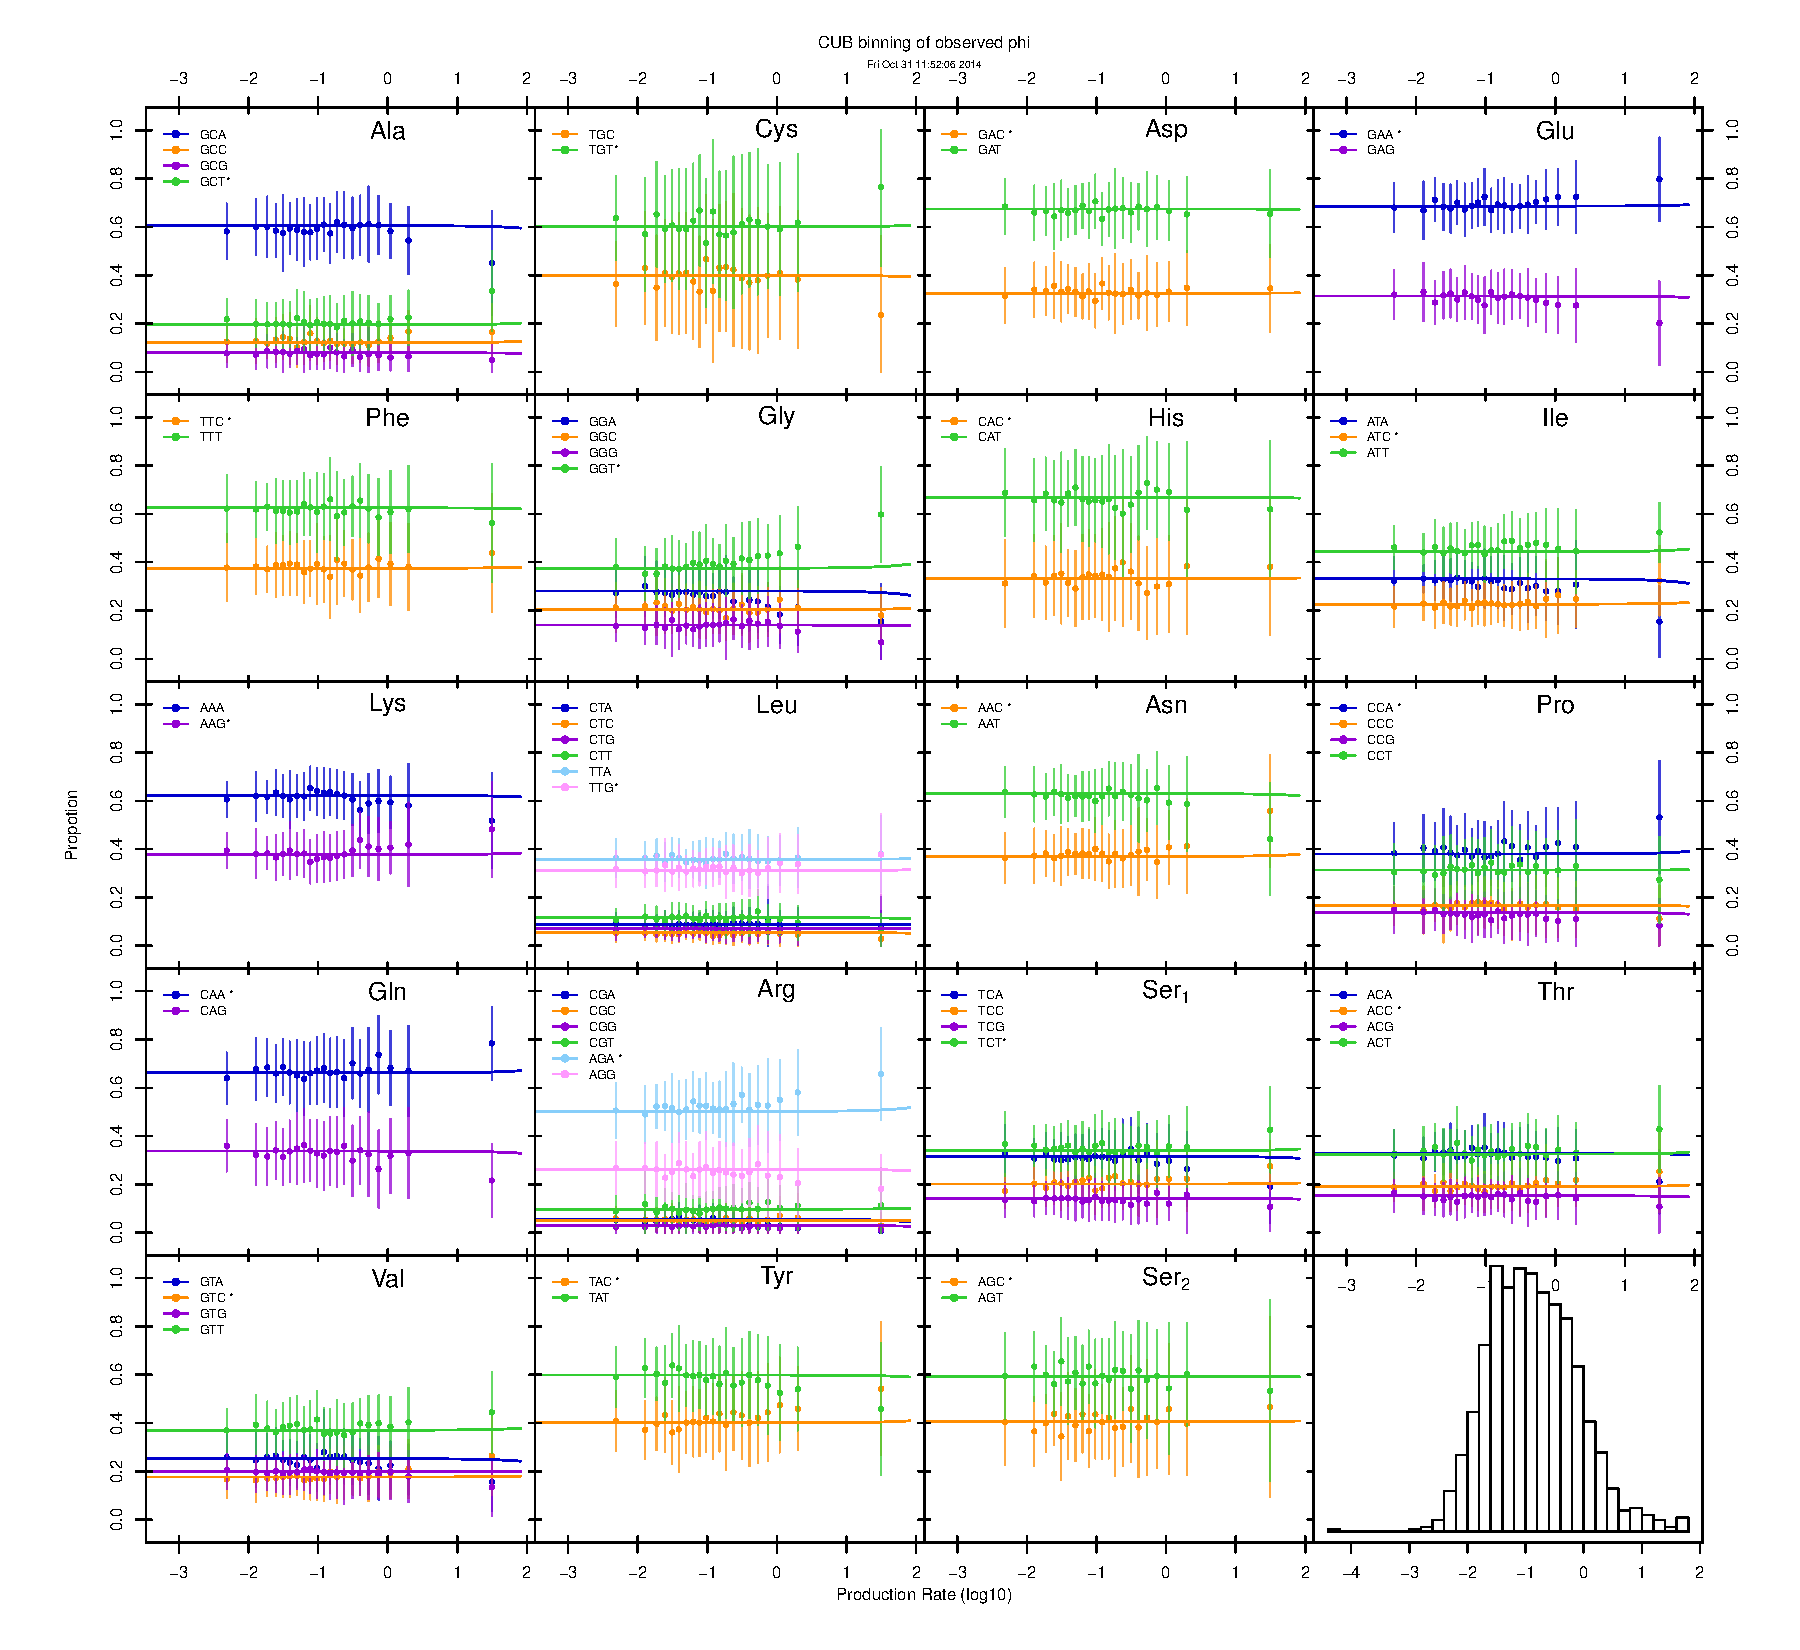
\includepdf[pages={1}]{data/oct31_CUB_obs_bin_NseYeast.pdf}
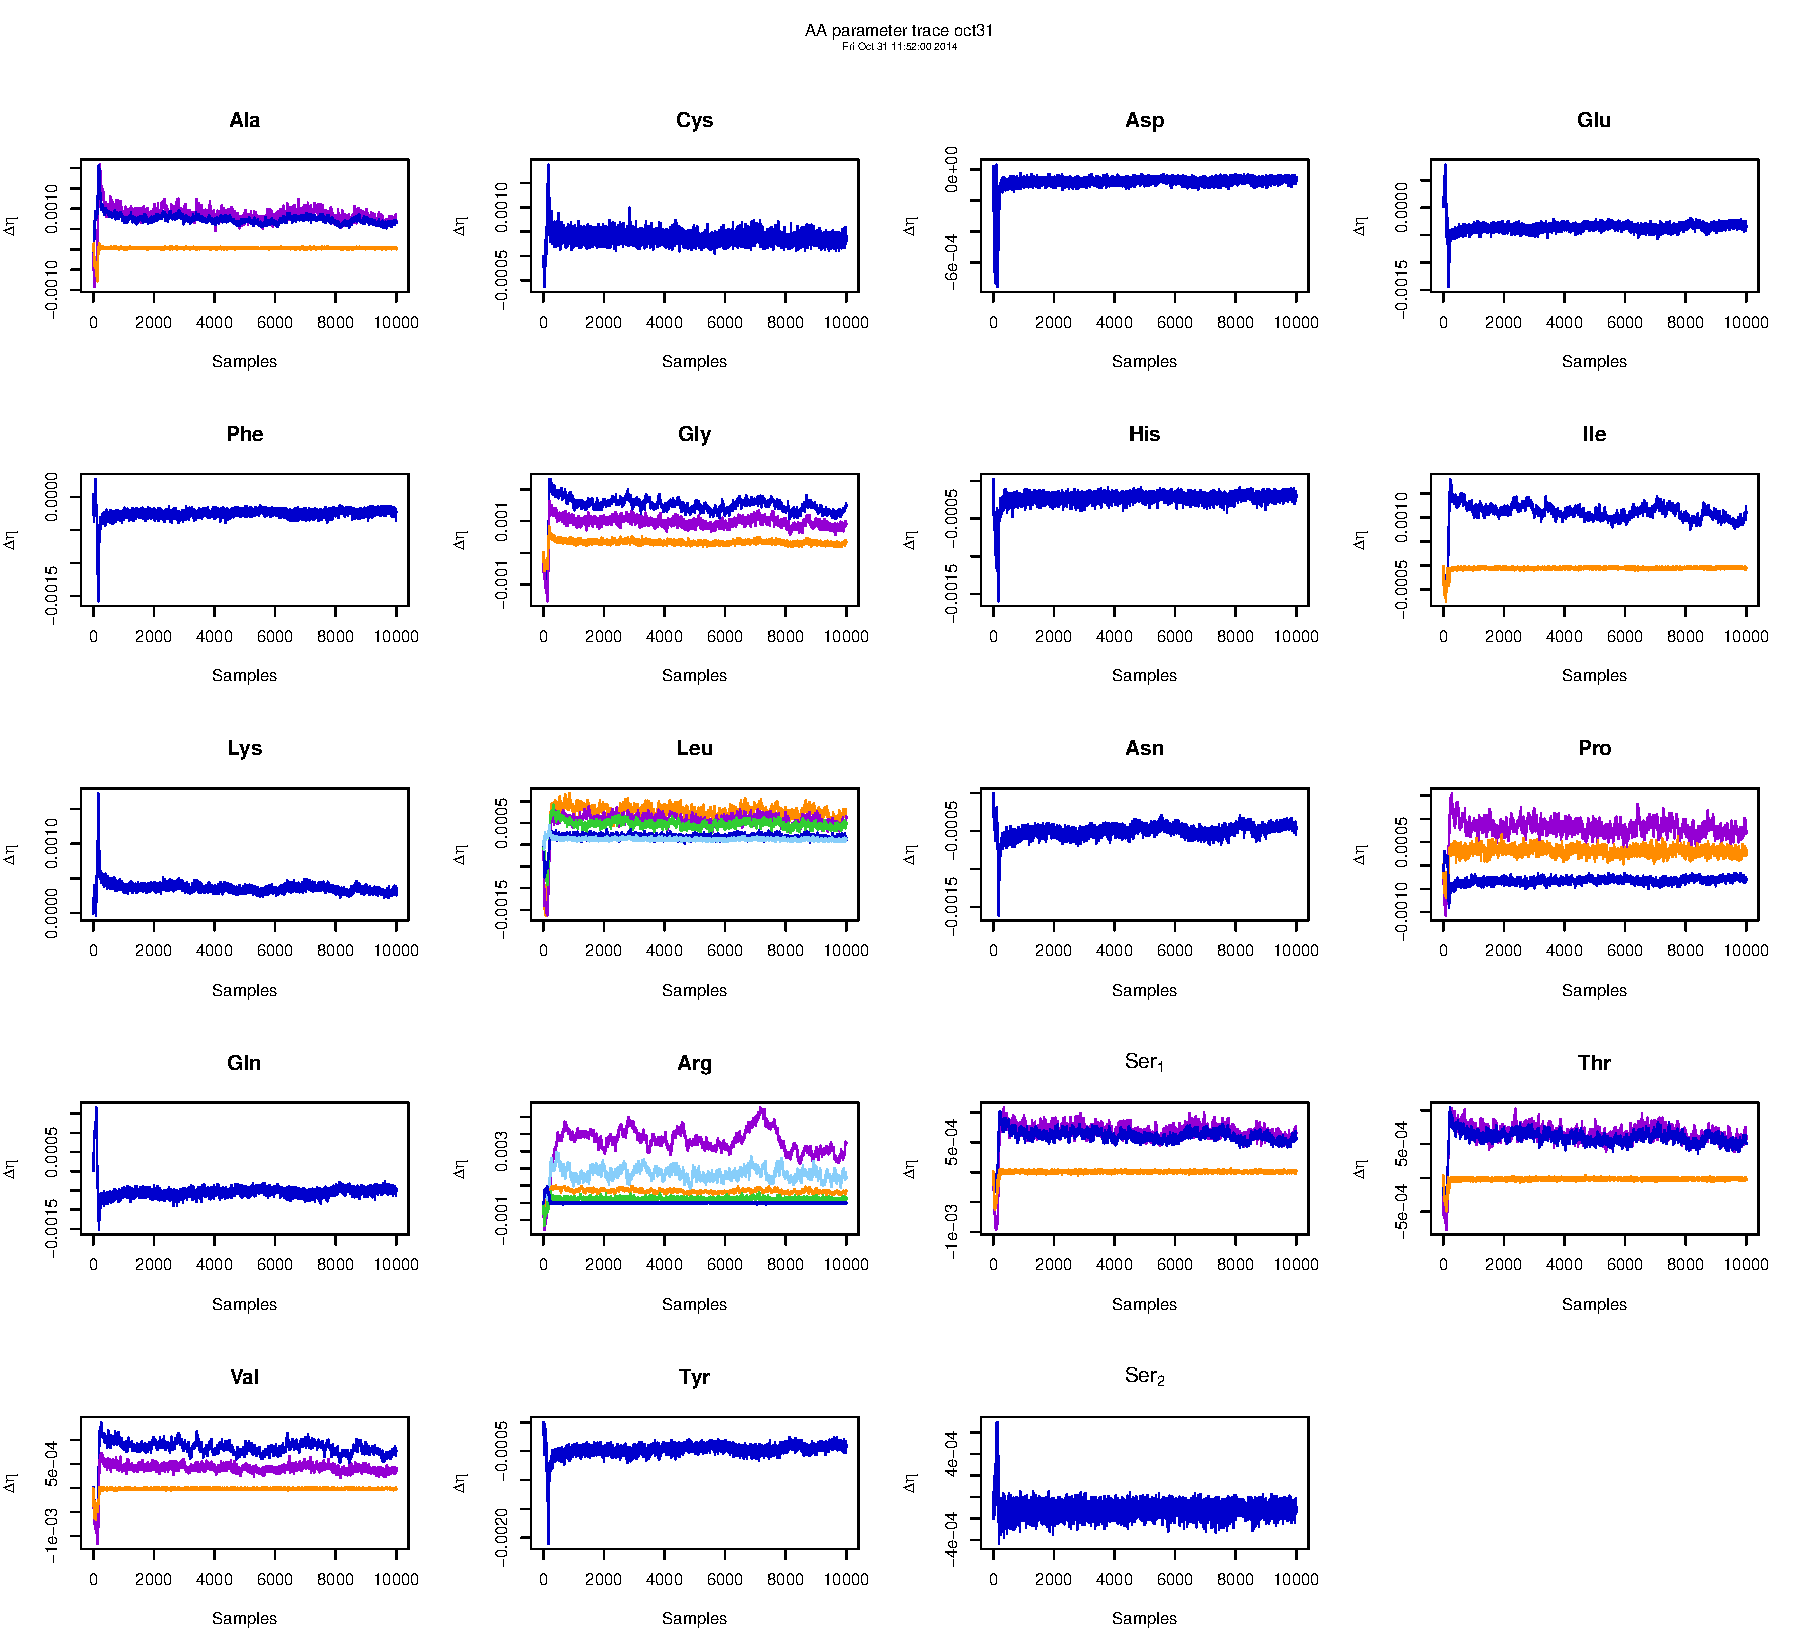
\includepdf[pages={1}]{data/oct31_deltaeta_NseYeast.pdf}
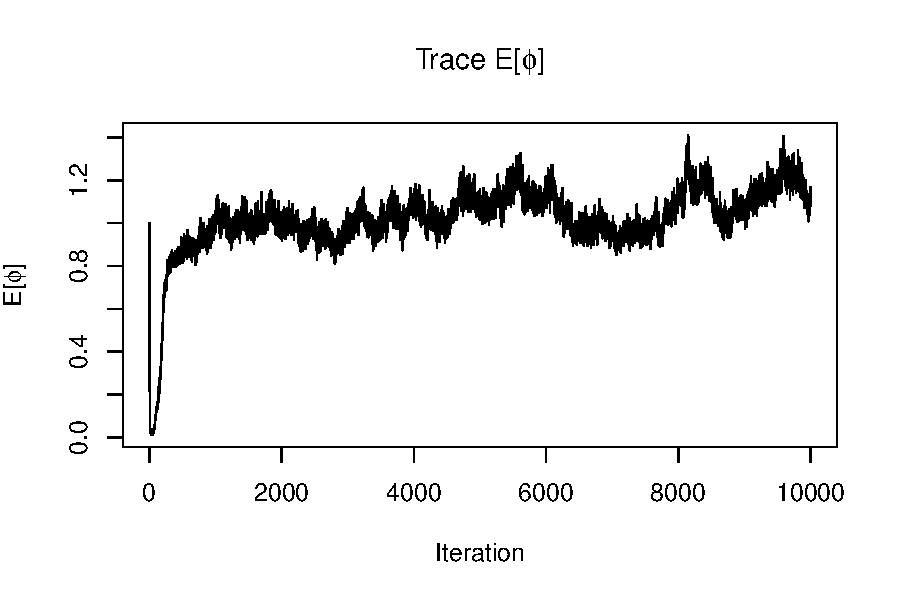
\includepdf[pages={1}]{data/oct31_expPhi_trace_NseYeast.pdf}
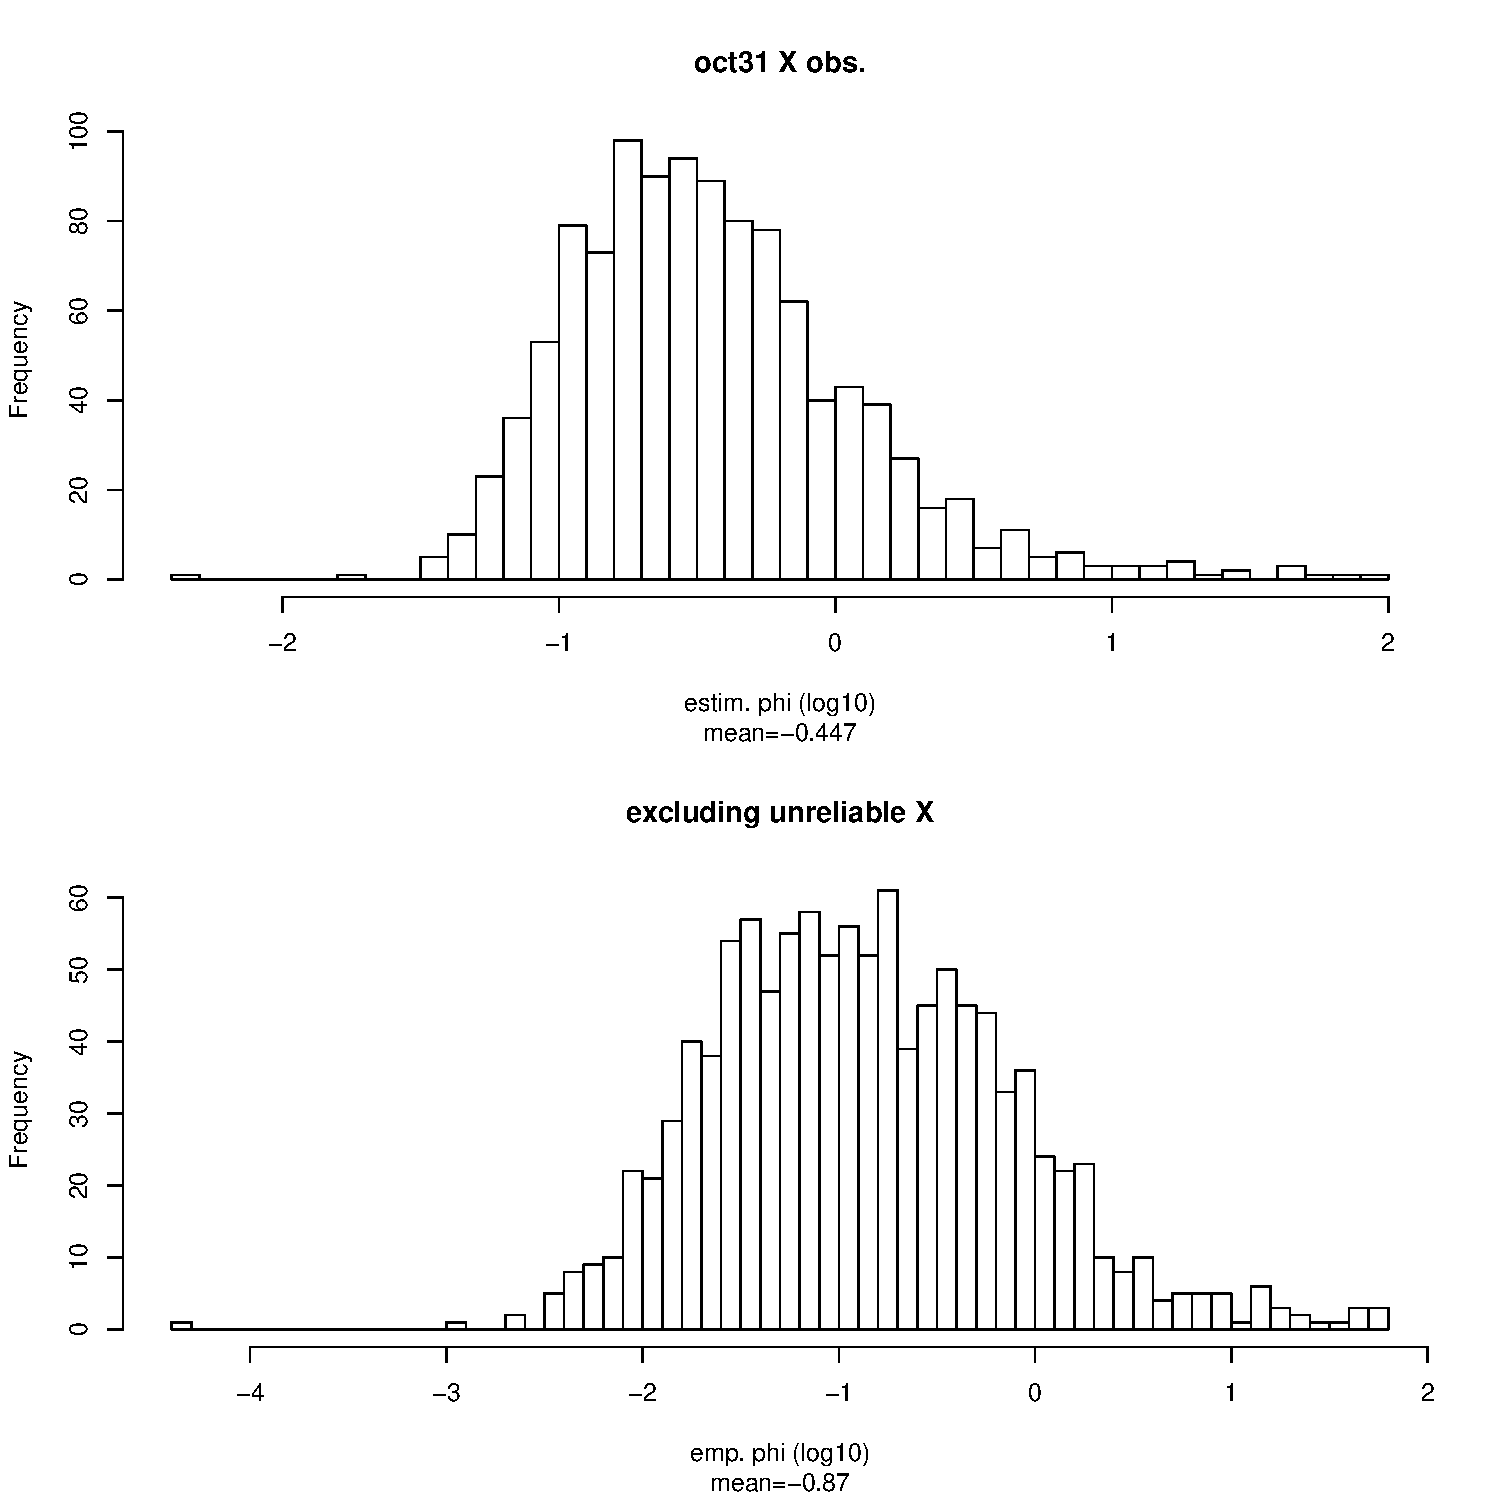
\includepdf[pages={1}]{data/oct31_histogram_NseYeast.pdf}
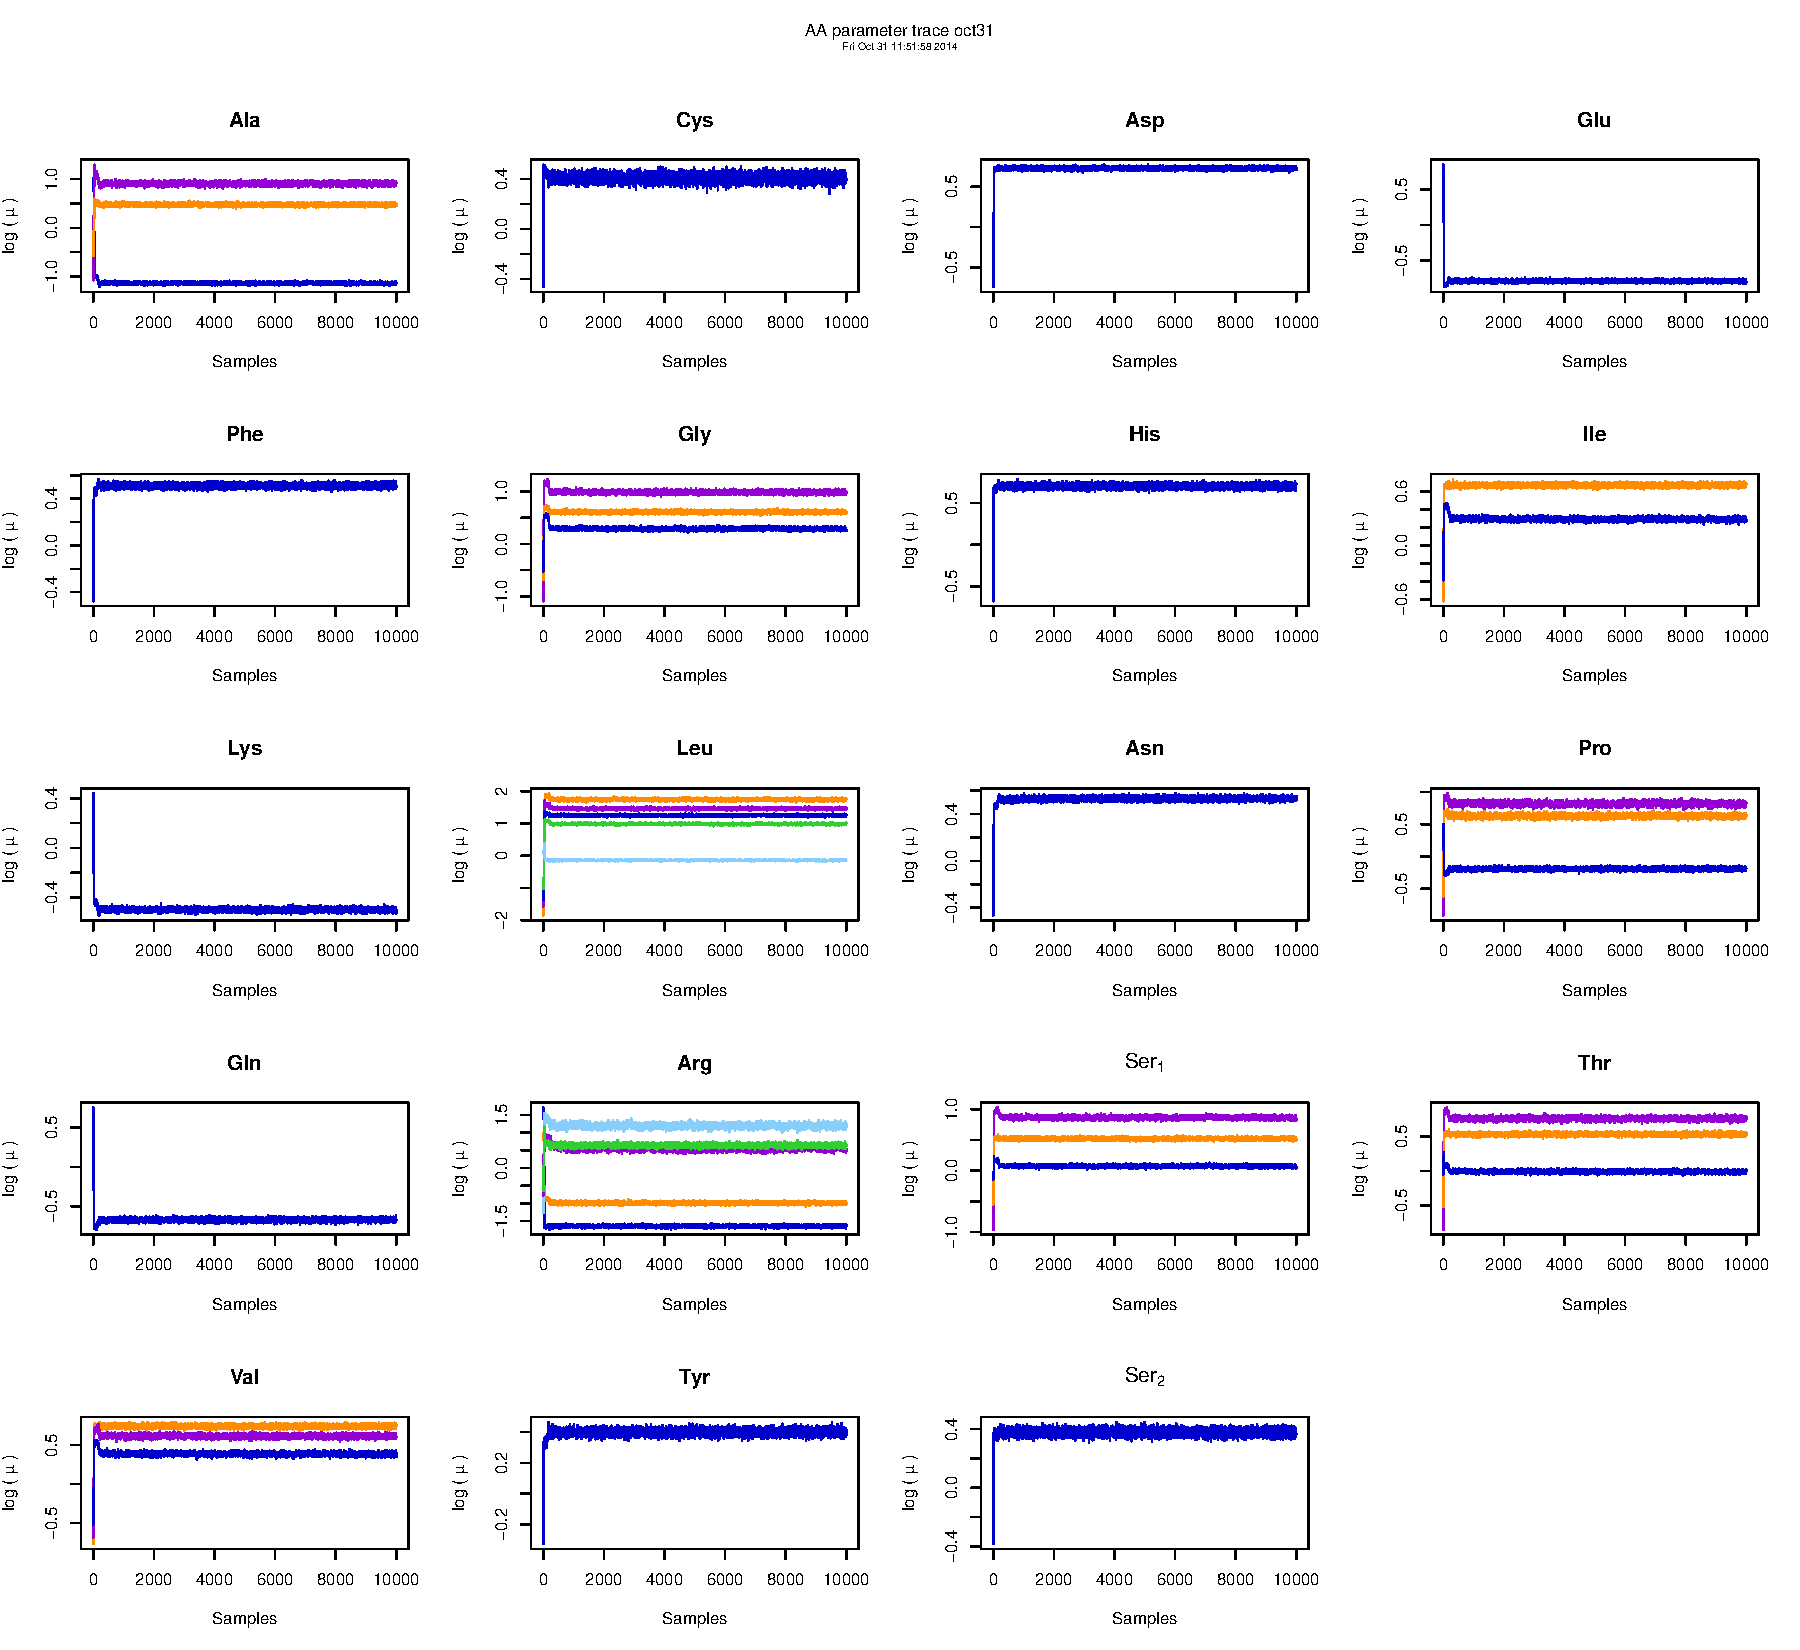
\includepdf[pages={1}]{data/oct31_logmu_NseYeast.pdf}
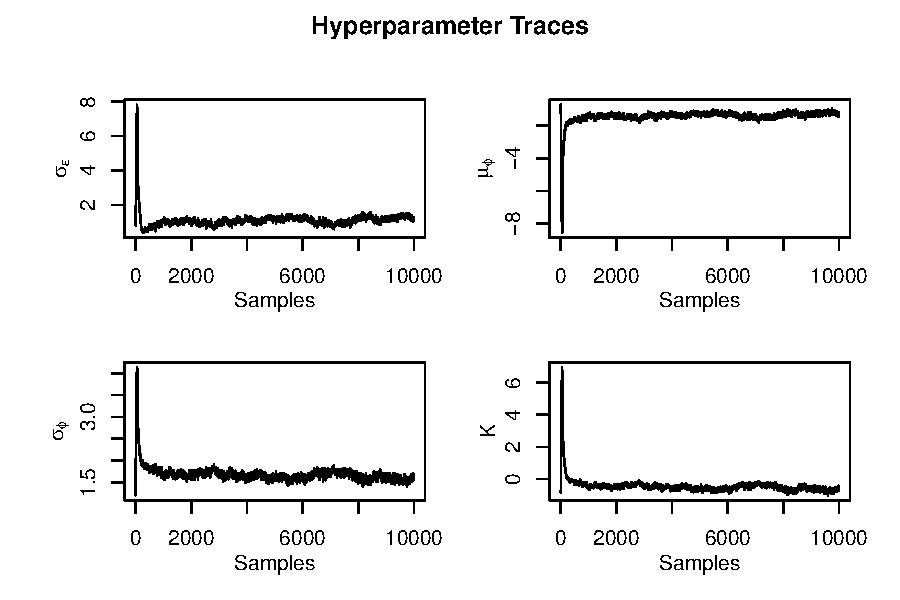
\includepdf[pages={1}]{data/oct31_pMat_trace_NseYeast.pdf}
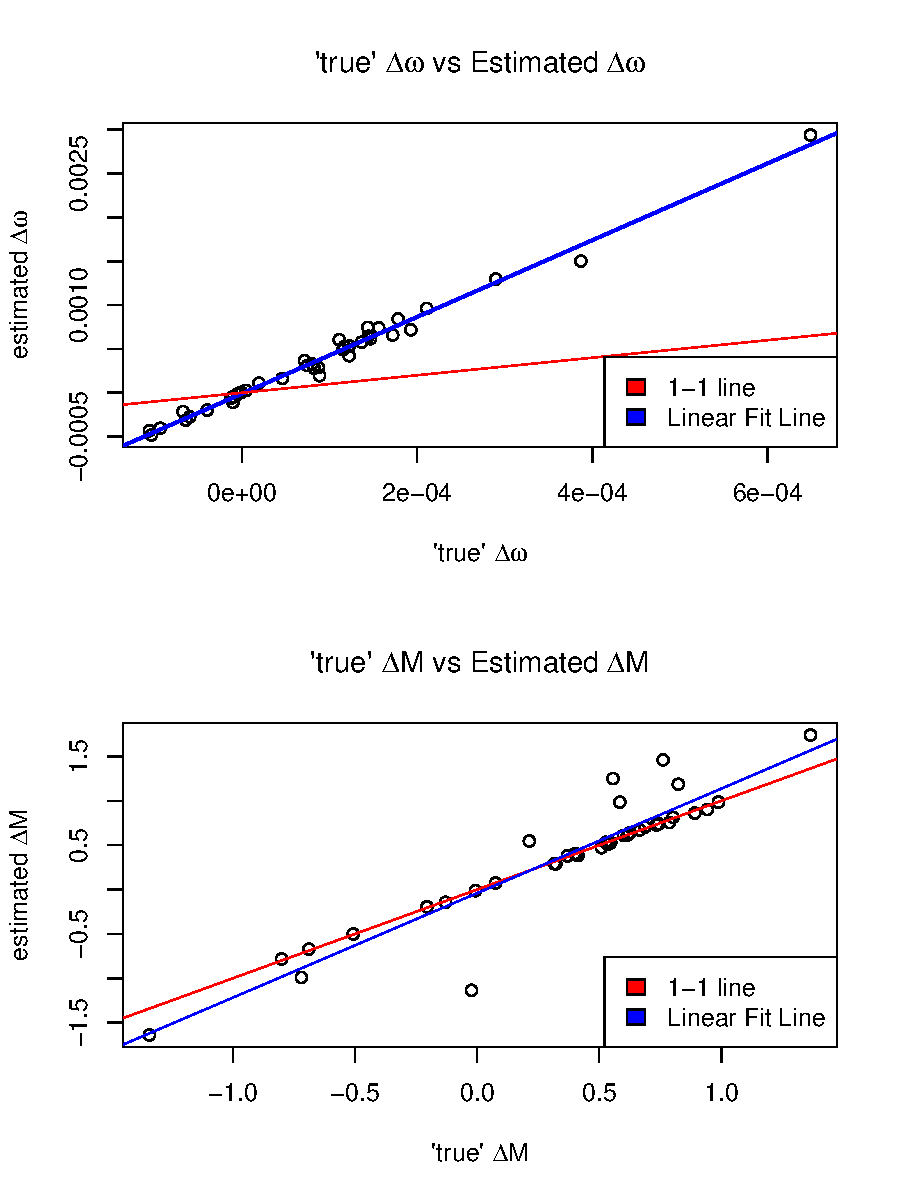
\includepdf[pages={1}]{data/oct31_results_NseYeast.pdf}
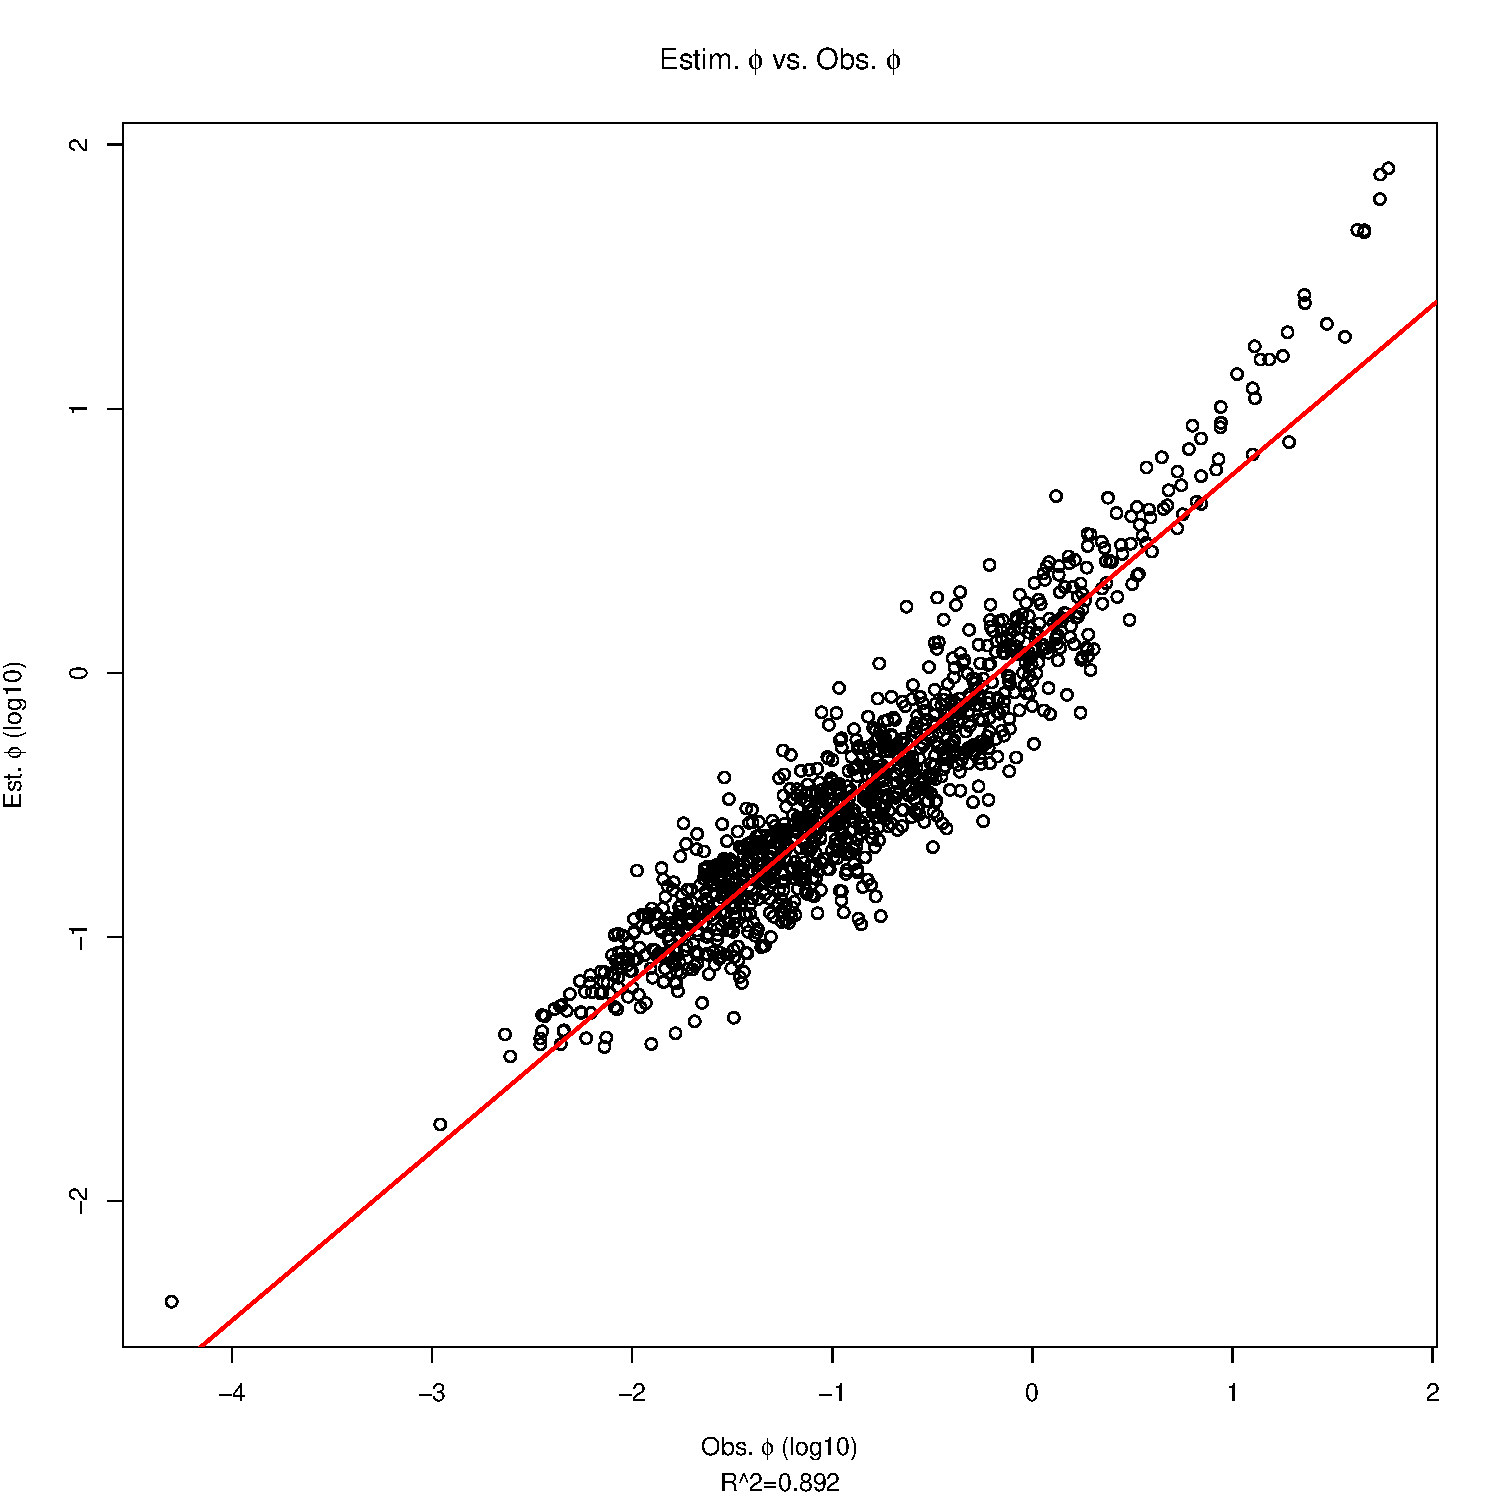
\includepdf[pages={1}]{data/oct31_vs_obs_phi_NseYeast.pdf}


\newpage
\subsection{Make a git repository for my scripts}

Done. https://github.com/ozway/cubmisc







\subsection{NSE Patches}

\subsubsection{Patch 1 - Avoiding the 6th iteration reset}

This is described in more detail in the section about stddev(phi), but I want to include the complete picture here.

These were the histograms of the Phi Scales before avoiding the 6th iteration reset. Note that the histogram on the left is actually of the Roc model for E Coli. Do not compare it to the Yeast histogram below.

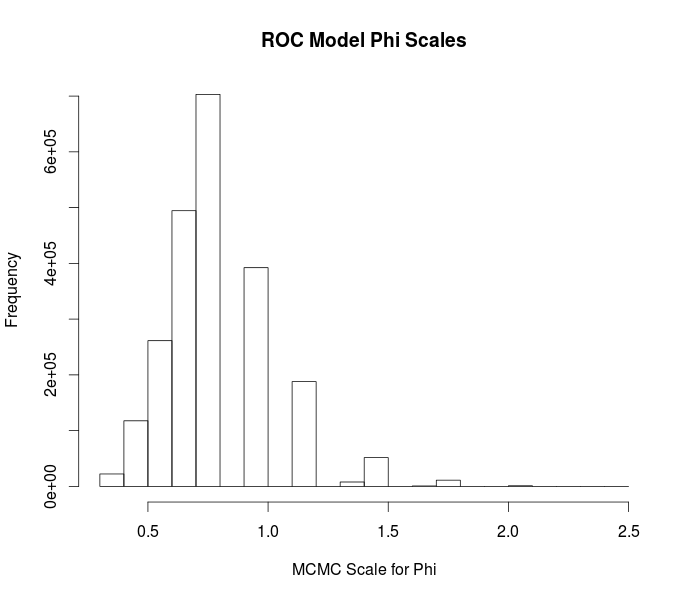
\includegraphics[width=0.5\textwidth]{data/oct10-roc-scalehist.png}
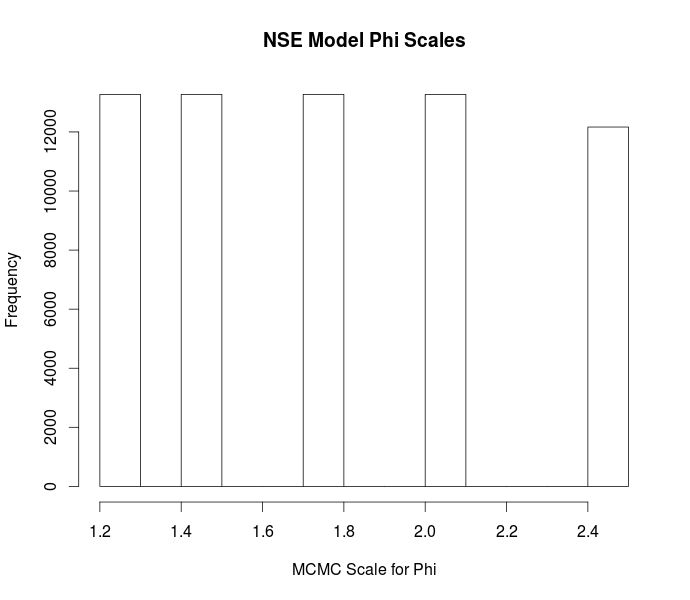
\includegraphics[width=0.5\textwidth]{data/oct10-nse-scalehist.png}


These are the updated histograms.

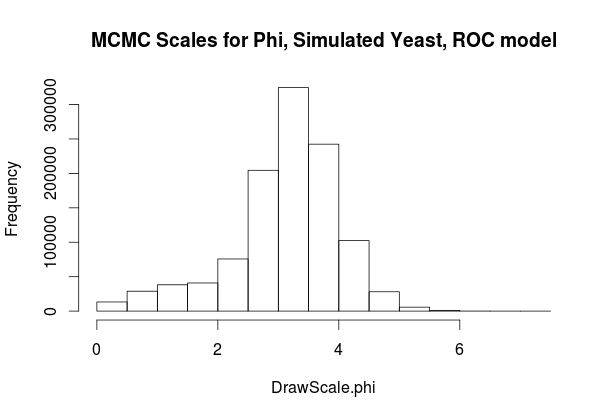
\includegraphics[width=0.5\textwidth]{data/oct17-RocYeastScales.png}
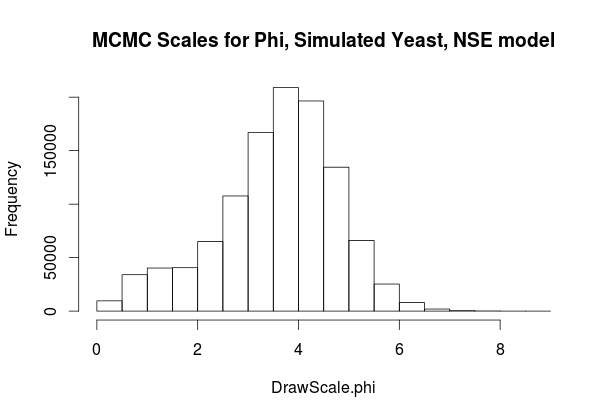
\includegraphics[width=0.5\textwidth]{data/oct17-NseYeastScales.png}

Here's a side-by-side comparison of RocYeast versus RocEcoli


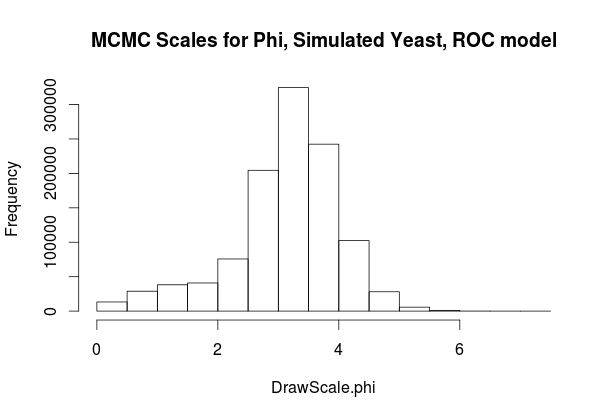
\includegraphics[width=0.5\textwidth]{data/oct17-RocYeastScales.png}
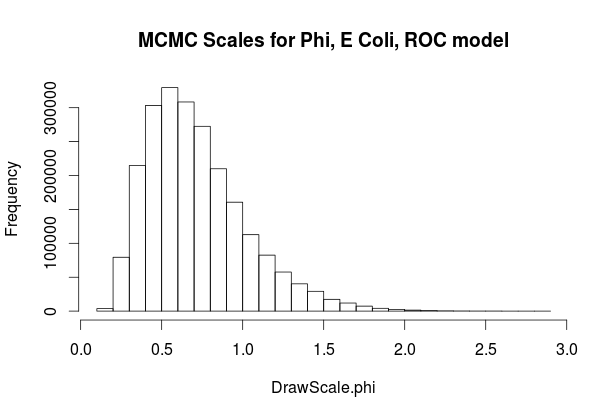
\includegraphics[width=0.5\textwidth]{data/oct20-RocEcoliScales.png}

\subsubsection{Patch 2 - Avoiding the Unending Scaling Loop}

I implemented C changes that replaced Wei-Chen's unending scaling loop with a one step subtraction. It seems that the code actually takes very slightly longer (.00013\% longer). My best explanation is that these operations were not taking up much time in the first place, so any differences is runtime were overtaken by the innate differences in the runtime (due to randomness).

\begin{verbatim}
                  Before Change   After Change
(total time)          124806.34      125446.36
my.inverse.mlogit      50367.20       50641.80
.Call                  41140.64       41373.00
match                  10364.14       10441.72
is.nan                  4784.92        4809.60
%*%                     4507.52        4536.28
<Anonymous>             3497.62        3548.08
cbind                   3444.98        3448.48
matrix                  2634.48        2633.28
cat                     1750.56        1720.10
\end{verbatim}

If further testing confirms this, I may revert the change, giving Wei-Chen's code the benefit of the doubt.

More problematic is that this still doesn't fix the important problem, values going to NaN causing the acceptance step to crash.


\subsubsection{Patch 2a - Everything-max\_exp}

Subtract out max\_exp from everything, all the time.
Definitely forces everything $<=$ 0;

Only concern is that if something small is there, it will be forced too low, and be exponentiated to 0. Not a LARGE concern, but a concern.

Also, I think I've figured out why the old code didn't fix the problem.

It evaluated $1459461302749408768.000000 - 709.782713 = 1459461302749408000.000000$. This is some sort of arithmetic error in C. It simplifies this sort of subtraction for questionable reasons. This causes the scaled high value to take values larger than ln(DBL\_MAX). This lead to an infinite exponent, which caused NaN normalized values.

The new code still suffers from a version of this problem, but not in a way that will crash the code. 

1459461302749408\textbf{638}.000000 rounds to
1459461302749408\textbf{512}.000000

Values seem to be going up and down to nearby values such that max-value is a sum of (powers of two of at least 256). If the difference is 1111, the second value changes so that the difference is 1024. If the difference is 1000, it rounds to 512. if the difference is 800, it goes to a difference of 768. differences of 129 or higher go to at least -256, and $e^{-256} \approx 0$. Differences of 128 or lower go to 0.  If the phi values differ by 129 orders of magnitude, then one of them simplifying to 1 and the other simplifying to 0 is not overly concerning. There is a loss of precision when there is a difference of 1-128, where they get proposed at 50\% each, but for values this high ($10^{18}$), the loss of precision can likely be ignored.


In any case, max-max always comes back 0, and since everything else is below max, everything should be in an exponentiable range. The only problem is that the things that aren't the max value 

\subsubsection{Patch 3 - Fix how the .Bmat file is written}

One concern that I have is that the bmat files are being badly written for the NSE model. They should look like 

\begin{verbatim}
Parameter,Value,SD
A,0.601255504722893,0.0237033066067192
A,1.13452224653582,0.0267133181736158
A,1.30103073124409,0.0238480349000172
A,-0.318856124276582,0.0185921125022695
A,-0.638707250936925,0.0239128208157251
A,-0.430302895729612,0.0198676086998986
C,-0.0281672064573597,0.050965967492386
C,0.306346224638228,0.0485649142612776
D,-1.04923142474412,0.0247797820471684
D,0.548947123948893,0.0217844280815052
\end{verbatim}

However, they look like this

\begin{verbatim}
Parameter,Value,SD
(Intercept):1,-1.13368719411271,0.0163254262432022
(Intercept):2,0.474079558190101,0.0187917078911786
(Intercept):3,0.898302427488134,0.0273650691145686
tmp.phi:reu13.df.aa$Pos:1,0.000638113297651608,3.70900280679152e-05
tmp.phi:reu13.df.aa$Pos:2,2.66219626036282e-05,9.17596078252389e-06
tmp.phi:reu13.df.aa$Pos:3,0.000762697807068617,7.47917510033425e-05
(Intercept),0.407527027594279,0.0285214413558274
tmp.phi:reu13.df.aa$Pos,0.000319785184813285,8.90451644378058e-05
(Intercept),0.728372367207557,0.0119226668866337
tmp.phi:reu13.df.aa$Pos,-6.65911530134893e-05,1.09884115801929e-05
\end{verbatim}


I'm fairly sure that this is some part of the code that is just getting the names of the codons wrong, however, I can't be sure. If deprecated part of the NSE code is reading the data structure incorrectly, then anything is possible. I want to fix this at one point.

10/31 update: I was right, the problem is just in cedric.mapBMatNames.r, he only attempts to write b.Mat names for the ROC model. For now, I've just copypasted the same naming functions from the roc model for the NSE model. I think if I use the browser to check out those values, I'll be okay.




\section{Goals for next Month}
\begin{enumerate}
\item Use Preston's Simulated Yeast, compare to REU yeast 

look for estimated $\approx$ 4*true
\item Parallelize the Code 

mclapply, getOption("mc.cores")?
\item Wei Chen's Yeast / Real Yeast Genome
\item Generate my own simulated yeast, using a reverse engineered cubfits
\end{enumerate}


\end{document} %End of day document, REMOVE
